\documentclass[dvipdfmx, 12pt]{beamer}
\usepackage{pxjahyper}
\usepackage{minijs}
\usepackage{otf}
\renewcommand{\kanjifamilydefault}{\gtdefault}
\usetheme{Dresden}
\setbeamertemplate{navigation symbols}{}
\usepackage{url}
\usepackage{graphicx}
\usepackage{comment}
\usepackage{amsmath}
\newenvironment<>{varblock}[2][.9\textwidth]{%
  \setlength{\textwidth}{#1}
  \begin{actionenv}#3%
    \def\insertblocktitle{#2}%
    \par%
    \usebeamertemplate{block begin}}
  {\par%
    \usebeamertemplate{block end}%
  \end{actionenv}}


\title{LEVEL-k AUCTIONS: CAN A NONEQUILIBRIUM MODEL OF STRATEGIC THINKING EXPLAIN THE WINNER'S CURSE AND OVERBIDDING IN PRIVATE-VALUE AUCTIONS?}
\author{Kei Ikegami}

\begin{document}
\newcommand{\argmin}{\mathop{\rm arg~min}\limits}

\frame{\maketitle}

\section*{Index}
	\begin{frame}\frametitle{Index}
	\tableofcontents
	\end{frame}

\section{Introduction}
	\begin{frame}\frametitle{Purpose}
	\end{frame}
	
	\begin{frame}\frametitle{Precedents}
	\end{frame}
	
	\begin{frame}\frametitle{What's new}
	\end{frame}
	
	\begin{frame}\frametitle{Result}
	\end{frame}
	
\section{Models}
	\subsection{Overview}
		\begin{frame}\frametitle{General Model}
			\begin{itemize}
			\item $N$ bidders bid for a single object.
			\item $X_i$ is bidder $i$'s private signal. $X = (X_1, \dots, X_N)$.
			\item $S_j$ is additional random variable which is informative about the value of the object. $S = (S_1, \dots, S_M)$.
			\item $V_i = u_i(S, X)$ is bidder $i$'s value of the object, where $u_i$ is symmetric across $i$.
			\item $V_i - p$ is the payoff for the bidder $i$ winning the auction by paying $p$.
			\item $Y$ is the highest signal among bidders other than $i$.
			\item $\upsilon(x, y) = E\left[ V_i | X_i = x, Y = y \right]$ is the expected value conditional on winning.
			\item $r(x) = E\left[ V_i | X_i = x \right]$ is the unconditional expected value.
			\end{itemize}
		\end{frame}
		
		\begin{frame}\frametitle{Classification of Auctions}
			\begin{itemize}
			\item First price auction vs Second price auction
			\item Independent private value auction(i.p.v) vs Common value auction(c.v)
			\item In i.p.v, the signals and values are independent among bidders. And then $\upsilon(x,x) = r(x) = x$.
			\item In c.v, the information of $i$ and $j$ is not independent and learning about the other bidders' information can cause the bidder to reassess his estimate of the value of the object (e.g. Timber auction). And so $\upsilon(x,x) \neq r(x)$ normally with $r(x) > \upsilon(x,x)$.
			\end{itemize}
		\end{frame}
		
	\subsection{Equilibrium}
		\begin{frame}[shrink]\frametitle{First Price Auction}
			\begin{itemize}
			\item In c.v, the optimal bidding strategy is calculated as (1).
			\item In i.p.v, the optimal bidding strategy is calculated as (2), because $\upsilon(x,x) = x$ and $Y$ is independent of $X$.
			\item Using $\upsilon(x,x)$ is called "value adjustment for the information revealed by winning".
			\item The latter terms in (1) and (2) are due to "bidding trade-off", which means higher bidding raises both the probability of winning and the cost.
			\end{itemize}
			
			\begin{align}
				a_*(x) &= \upsilon(x, x) - \int_{\underline{x}}^{x} \exp \left( -\int_{y}^{x} \frac{f_Y(t|t)}{F_Y(t|t)} \mathrm{d}t \right) \mathrm{d} (\upsilon(y,y)) \\[10pt]
				a_*(x) &= x - \int_{\underline{x}}^{x} \frac{F_Y(y)}{F_Y(x)} \mathrm{d}y
				= E\left[ Y | Y < X \right]
			\end{align}
						
		\end{frame}
		
		\begin{frame}\frametitle{Second Price Auction}
			\begin{itemize}
			\item In c.v, the optimal bidding strategy is calculated as (3). This is not a weakly dominant strategy.
			\item In i.p.v, the optimal bidding strategy is calculated as (4), because $\upsilon(x,x) = x$. This is a weakly dominant strategy.
			\end{itemize}
			
			\begin{align}
				b_*(x) &= \upsilon(x,x) \\
				b_*(x) &= x
			\end{align}
			
		\end{frame}
		
	\subsection{Cursed Equilibrium}
		\begin{frame}[shrink]\frametitle{Points}
			\begin{itemize}
			\item $\chi$ is the parameter denoting the probability that the bidder think the other bidders bid independently of signals. 
			\item Cursed equilibrium for a given $\chi$ value is called $\chi$-cursed equilibrium.
			\item In ER's(2002, 2006), $\chi$-cursed equilibrium is the same as one in a hypothetical "$\chi$-virtual game", in which players believe that, with probability $\chi$, other's bid is independent of types.
			\item In i.p.v, the players bid independently of others' signals by definition, then the optimal bidding strategy in $\chi$-cursed equilibrium is the same as one in equilibrium ($\upsilon(x, x) = r(x) = x$).
			\item In c.v, since $\upsilon(x,x) \neq r(x)$, cursed equilibrium differs from equilibrium.
			\end{itemize}
		\end{frame}
		
		\begin{frame}\frametitle{Common Value Auction}
			\begin{itemize}
			\item In first price auction, the optimal bidding strategy is calculated as (5).
			\item In second price auction, the optimal bidding strategy is calculated as (6).
			\item These calculations are exactly the same as ones in equilibrium.
			\end{itemize}
			
			\footnotesize
			\begin{align}
				a_{\chi}(x) &= \left\{ (1 - \chi)\upsilon(x,x) + \chi r(x) \right\} \nonumber \\
				&\quad - \int_{\underline{x}}^x \exp \left( - \int_y^x \frac{f_Y(t|t)}{F_Y(t|t)} \mathrm{d}t \right) \mathrm{d}\left\{ (1 - \chi)\upsilon(y,y) + \chi r(y) \right\} \\
				b_{\chi}(x) &= (1 - \chi)\upsilon(x,x) + \chi r(x)
			\end{align}
			\normalsize
			
		\end{frame}
		
	\subsection{Nonequilibrium Level-k Models}
		\begin{frame}[shrink]\frametitle{Points}
			\begin{itemize}
			\item Level-k model allows behavior to be heterogeneous, but assumes that each player's behavior is drawn from the common distribution over the k types.
			\item In this paper there are 3 types (denoted by L k) which best response to the lower type. i.e. L1 best responses to L0, and L2 best responses to L1.
			\item The key assumption is the behavior of L0.  One is Random L0, in which the L0 bids uniformly randomly independent of its own signal. The other is Truthful L0, in which L0 bids the value suggested by its own signal.
			\item L1 and L2 are called Random L1 and L2 when L0 is set to Random L0.
			\item L1 and L2 are called Truthful L1 and L2 when L0 is set to Truthful L0. 
			\item In the latter slides I show the optimal bidding strategies of each player in each case one by one.
			\end{itemize}
		\end{frame}
		
		\begin{frame}\frametitle{Random L0}
			\begin{itemize}
			\item This player bids i.i.d. uniformly over the range $[\underline{z}, \bar{z}]$, which is determined by its private signal and the value $V_i = u_i (S, X)$.
			\end{itemize}
		\end{frame}
		
		\begin{frame}\frametitle{Random L1 in First Price Auction}
			\begin{itemize}
			\item Random L1 plays in the belief that all other players follow Random L0. 
			\item Let $Z$ be the highest bid among the others, the distribution function of $Z$ be $F_z (z)$, and the pdf be $f_z(z)$ (these two are from the ordered statistics).
			\item The optimal bidding strategy of Random L1 ($a_1^r(x)$) solves (7) and is characterized by (8).
			\end{itemize}
			
			\begin{align}
				\max_a \int_\underline{z}^a (r(x) - a) f_z(z) \mathrm{d}z \\
				(r(x) - a)f_z(a) - F_z(a) = 0
			\end{align}
		\end{frame}
		
		\begin{frame}\frametitle{Random L1 in First Price Auction}
			\begin{itemize}
			\item This optimal bidding strategy is common in i.p.v and c.v.
			\item There are two differences from the optimal bidding strategy in equilibrium.
			\item One is that $r(x)$ replaces $\upsilon(x,x)$, which reflects the fact that Random L1 think winning conveys no information about the value of the object even in c.v. (difference in value adjustment). Since in general $r(x) > \upsilon(x,x)$, Random L1 tends to overbid due to the value adjustment.
			\item Second is that the integral in (7) is over $Z$ rather than $Y$ (see (1) in paper). This is caused by L1 use nonequilibrium belief to evaluate the bidding trade-off.  (difference in bidding trade-off)
			\end{itemize}
		\end{frame}
		
		\begin{frame}\frametitle{Random L1 in Second Price Auction}
			\begin{itemize}
			\item The optimal bidding strategy ($b_1^r(x)$) solves (9)'s maximization problem. And get (10).
			\end{itemize}
			
			\begin{align}
				&\max_b \int_\underline{z}^b (r(x) - z) f_z(z)\mathrm{d}z\\
				&b_1^r(x) = r(x)
			\end{align}
		\end{frame}
		
		\begin{frame}\frametitle{Random L1 in Second Price Auction}
			\begin{itemize}
			\item One difference from equilibrium case is $r(x)$ replaces $\upsilon(x,x)$. (difference in value adjustment). And this leads to overbidding in c.v.
			\item Second difference from equilibrium case is that the player use nonequilibrium belief. However note that this does not result in the deviating from truthful bidding as in first price auction.
			\item In other words, we have no bidding trade-off term in the optimal bidding strategy just as in the equilibrium case.
			\item (10) coincides with (6) when $\chi = 1$, i.e. fully cursed equilibrium.
			\item (10) coincides with equilibrium in i.p.v, where $r(x) = x$.
			\end{itemize}
		\end{frame}
		
		\begin{frame}\frametitle{Random L2 , Truthful L1 and Truthful L2}
			\begin{itemize}
			\item Random L2 best responses to Random L1.
			\item (8) and (10) tell that Random L1's bidding strategy is an increasing function of its private signal both in first and second price auction.
			\item For Random L2 in this case, the high bid among the other players conveys the information about the value of the object, then Random L2 adjust its own estimated value according to the information. This means that we use $\upsilon(x, y)$ rather than $r(x)$.
			\item This structure is common in Truthful L1 and Truthful L2. Thus I provide the general bidding strategy which can be applied to the three cases.
			\end{itemize}
		\end{frame}
		
		\begin{frame}\frametitle{General Bidding Strategy in First Price Auction}
			\begin{itemize}
			\item Suppose that a level-k bidder expects others to bid according to the monotonically increasing bidding strategy $a_{k-1}(x)$.
			\item The bidder's optimal bidding strategy with $V_i$ and $X_i$ solves (11), and is characterized by the first order condition (12). 
			\end{itemize}
			
			\footnotesize
			\begin{align}
				&\max_a \int_\underline{x}^{a_{k-1}^{-1}(a)} (\upsilon(x, y) - a) f_Y(y | x) \mathrm{y} \\
				&(\upsilon(x, a_{k-1}^{-1}(a)) - a)f_Y(a_{k-1}^{-1}(a) | x) \frac{\partial a_{k-1}^{-1}(a)}{\partial a} - F_Y(a_{k-1}^{-1}(a) | x) = 0
			\end{align}
			\normalsize
			
		\end{frame}
		
		\begin{frame}\frametitle{General Bidding Strategy in Second Price Auction}
			\begin{itemize}
			\item Suppose that a level-k bidder expects others to bid according to the monotonically increasing bidding strategy $b_{k-1}(x)$.
			\item The bidder's optimal bidding strategy with $V_i$ and $X_i$ solves (13), and is characterized by the first order condition (14). 
			\end{itemize}
			
			\begin{align}
				&\max_b \int_\underline{x}^{b_{k-1}^{-1}(b)} (\upsilon(x, y) - b_{k-1}(y)) f_Y(y | x) \mathrm{y} \\
				&b = \upsilon(x, b_{k-1}^{-1}(b))
			\end{align}
		\end{frame}
		
		\begin{frame}[shrink]\frametitle{Strategic Substitutability}
			\begin{itemize}
			\item What does mean "Value adjustment (using $\upsilon(x,x)$) tends to make bidders' bids strategic substitutes" ?
			\item level-kが、周囲の奴らが均衡よりもoverbidしていると考えているとする。
			\item この時、もしその状態(overbidの状態)が均衡だった時に想定される彼らのprivate signalよりも、実際に彼らが受け取っているprivate signalは小さい(弱い)と考えられる。
			\item その分のvalue adjustmentをlevel-k bidderが行う。この際の修正は、均衡bidよりも少し低いbidとなる。なぜなら質が周囲のbid状況から想定されるほど良くないぞという情報を受け取っているから。
			\item こうして、周囲がoverbidなら自分はunderbid、という戦略的代替が成り立つことがわかった。
			\end{itemize}
		\end{frame}
		
		\begin{frame}\frametitle{Random L2 in First Price Auction}
			\begin{itemize}
			\item $a_2^r(x)$ is determined by (12) with $a_1^{r^{-1}}(a)$ replacing $a_{k-1}^{-1}(a)$.
			\item Given the strategic substitutability of value adjustment, Random L2 underbid because Random L1 overbid relative to the equilibrium level.
			\end{itemize}
			
			\begin{align}
				(\upsilon(x, a_1^{r^{-1}}(a)) - a)f_Y(a_1^{r^{-1}}(a) | x) \frac{\partial a_1^{r^{-1}}(a)}{\partial a} - F_Y(a_1^{r^{-1}}(a) | x) = 0
			\end{align}
			
		\end{frame}
		
		\begin{frame}\frametitle{Random L2 in Second Price Auction}
			\begin{itemize}
			\item $b_2^r(x)$ is determined by (14) with $b_1^{r^{-1}}(b)$ replacing $b_{k-1}^{-1}(b)$.
			\item Given the strategic substitutability of value adjustment, Random L2 underbid because Random L1 overbid relative to the equilibrium level.
			\item Bidding strategy is again truthful ("truthful" means that the bidder does not consider the bidding trade-off).
			\item Note that $b_1^r(x) = r(x)$ from (10).
			\end{itemize}
			
			\begin{align}
				b = \upsilon(x, b_1^{r^{-1}}(b)) = \upsilon(x, r^{-1}(b))
			\end{align}
		\end{frame}
		
		\begin{frame}\frametitle{Truthful L1 in First Price Auction}
			\begin{itemize}
			\item Truthful L0's bidding strategy is denoted by $a_0^t(x) \equiv r(x)$, which is from the definition of Truthful L0.
			\item Truthful L1's bidding strategy ($a_1^t(x)$) can be characterized by the special case of (12) with $r(x)$ replacing $a_{k-1}(x)$.
			\item Since Truthful L0 overbids relative to the equilibrium (see (1)), the strategic substitutability tends to make Truthful L1 underbid. 
			\end{itemize}
			
			\begin{align}
				(\upsilon(x, r^{-1}(a)) - a)f_Y(r^{-1}(a) | x) \frac{\partial r^{-1}(a)}{\partial a} - F_Y(r^{-1}(a) | x) = 0
			\end{align}
			
		\end{frame}
		
		\begin{frame}\frametitle{Truthful L1 in Second Price Auction}
			\begin{itemize}
			\item The optimal bidding strategy of Truthful L1 ($b_1^t(x)$) can be characterized by (14) with $b_0^t(x) \equiv r(x)$ replacing $b_{k-1}(x)$. 
			\item Since Truthful L0 normally overbids relative to the equilibrium due to using $r(x)$ rather than $\upsilon(x,x)$, the strategic substitutability tends to make Truthful L1 underbid. 
			\end{itemize}
			
			\begin{align}
				b = \upsilon(x, r^{-1}(b))
			\end{align}
			
		\end{frame}
		
		\begin{frame}\frametitle{Truthful L2 in First Price Auction}
			\begin{itemize}
			\item By $a_1^t(x)$ replacing $a_{k-1}^t(x)$ in (12), the optimal bidding strategy ($a_2^t(x)$) is characterized.
			\item The strategic substitutability tends to make Truthful L2 overbid reflecting Truthful L1's underbidding. 
			\end{itemize}
			
			\begin{align}
				(\upsilon(x, a_1^{t^{-1}}(a)) - a)f_Y(a_1^{t^{-1}}(a) | x) \frac{\partial a_1^{t^{-1}}(a)}{\partial a} - F_Y(a_1^{t^{-1}}(a) | x) = 0
			\end{align}
			
		\end{frame}
		
		\begin{frame}\frametitle{Truthful L2 in Second Price Auction}
			\begin{itemize}
			\item By $b_1^t(x)$ replacing $b_{k-1}^t(x)$ in (14), the optimal bidding strategy ($b_2^t(x)$) is characterized.
			\item The strategic substitutability tends to make Truthful L2 overbid reflecting Truthful L1's underbidding. 
			\end{itemize}
			
			\begin{align}
				b = \upsilon(x, b_1^{t^{-1}}(b))
			\end{align}
			
		\end{frame}


\section{Comparing}
	\subsection{Optimal Bidding Strategy Comparing}
	
		\begin{frame}\frametitle{Auction Example: KL}
			\begin{itemize}
			\item KL(Kagel and Levin 1986) is an example of first price common value auction.
			\item $V_i = S$ is uniformly distributed on a subset of $[\underline{s}, \bar{s}]$.
			\item $X|S$ is conditionally uniformly i.i.d. on the interval $[s - \frac{a}{2}, s + \frac{a}{2}]$ with $a > 0$.
			\item Thus $f_{X|S} = \frac{1}{a}$ and $F_{X|S} = \frac{x-s}{a} + \frac{1}{2}$. And $E[X|S] = s$.
			\item Then the value adjustment for no information by winning is calculated as (21).
			\end{itemize}
			
			\begin{align}
				r(x) \equiv E[S|X = x] = x
			\end{align}
		\end{frame}
		
		\begin{frame}\frametitle{Derivation of (21)}
			Let the range of $S$ be $R_S$ and its length be $l_S$.
			\footnotesize
			\begin{align}
			E[S | X = x] &= \int_{R_S} s\cdot f_{S|X = x}(s) \mathrm{d}s = \int_{R_S} S \frac{f_{X=x|S}(x) f_S(s)}{\int_{R_S} f_{X=x|S}(x) f_S(s) \mathrm{d}s} \mathrm{d}s
			\end{align}
			\normalsize
			Now $\int_{R_S} f_{X=x|S}(x) f_S(s) \mathrm{d}s = \int_{x-\frac{a}{2}}^{x + \frac{a}{2}} \frac{f_S(s)}{a} \mathrm{d}s = \frac{1}{a\cdot l_S} a = \frac{1}{l_S}$
			\par
			Then
			\begin{align*}
			(22) &= \int_{R_S} s\cdot l_S\cdot f_{X=x|S}(x) f_S(s) \mathrm{d}s = \int_{R_S} s\cdot f_{X=x|S}(x) \mathrm{d}s\\
			&= \frac{1}{a}\int_{x-\frac{a}{2}}^{x + \frac{a}{2}} s\ \mathrm{d}s = \frac{1}{a}ax = x
			\end{align*}
		\end{frame}
		
		\begin{frame}\frametitle{Auction Example: KL}
			\begin{itemize}
			\item The value adjustment for the information revealed by winning is calculated as in (23).
			\item The derivation of (23) is in the web appendix.
			\item With $N > 2$, $\upsilon(x,x) \leq r(x) = x$\ holds. Thus the cursed equilibrium bidders overbid relative to the equilibrium.
			\end{itemize}
			\footnotesize
			\begin{align}
			\upsilon(x, y) = \begin{cases}
							x - \frac{a}{2} + \frac{a}{N} - \frac{x-y}{N} & x-a \leq y \leq x \\[10pt]
							y -\frac{a}{2} + \frac{a}{N} - \frac{\left( \frac{y-x}{a} \right)^{N-1}}{1-\left( \frac{y-x}{a} \right)^{N-1}} \left( \frac{N-1}{N} \right) (x + a- y) & x < y \leq x+a
						\end{cases}
			\end{align}
			\normalsize
		\end{frame}
		
		\begin{frame}[shrink]\frametitle{Auction Example: AK}
			
			\begin{itemize}
			\item AK (Avery and Kagel 1997) is an example of second price common value auction.
			\item $V_i = \sum_{i=1}^N X_i$, with $X_i$ i.i.d. uniformly distributed on the interval $[\underline{x}, \bar{x}]$.
			\item Each value adjustment can be calculated as follows.
			\item $\upsilon(x,x) > (<) r(x) \Leftrightarrow x > (<) \frac{(N-1)\bar{x} + \underline{x}}{N}$. i.e. $\upsilon(x,x) > r(x)$ with high signals and $\upsilon(x,x) < r(x)$ with low signals.
			\item Then, in cursed equilibrium, high signal bidders underbid relative to equilibrium and low signal bidders overbid relative to equilibrium.
			\end{itemize}
			
			\begin{align}
				r(x) &= x + (N - 1)\frac{\bar{x} + \underline{x}}{2} \\[10pt]
				\upsilon(x,y) &= x + y\frac{N}{2} + \frac{N-2}{2}\underline{x}
			\end{align}
		\end{frame}
		
		\begin{frame}\frametitle{Auction Example: AK}
			\begin{itemize}
			\item In AK, $N$ is set to be $2$ and $[\underline{x}, \bar{x}] = [1, 4]$.
			\item Thus $r(x) = x + \frac{5}{2}$ and $\upsilon(x,x) = 2x$.
			\item $r(x) < \upsilon(x,x)$ when $x > \frac{5}{2}$.
			\item $r(x) > \upsilon(x,x)$ when $x < \frac{5}{2}$. 
			\end{itemize}
		\end{frame}
		
		\begin{frame}\frametitle{Auction Example: GHP}
			\begin{itemize}
			\item GHP (Goeree, Holt, and Palfrey 2002) is an example of independent private value first price auction.
			\item $N = 2$ and $V_i = X_i$.
			\item In a low-value treatment, bids are restricted to $\left\{ 0,2,4,6,8,11 \right\}$ with equal probability for each.
			\item In a high-value treatment, bids are restricted to $\left\{ 0,3,5,7,9,12 \right\}$ with equal probability for each.
			\end{itemize}
		\end{frame}
		
		\begin{frame}\frametitle{Summary Table}
			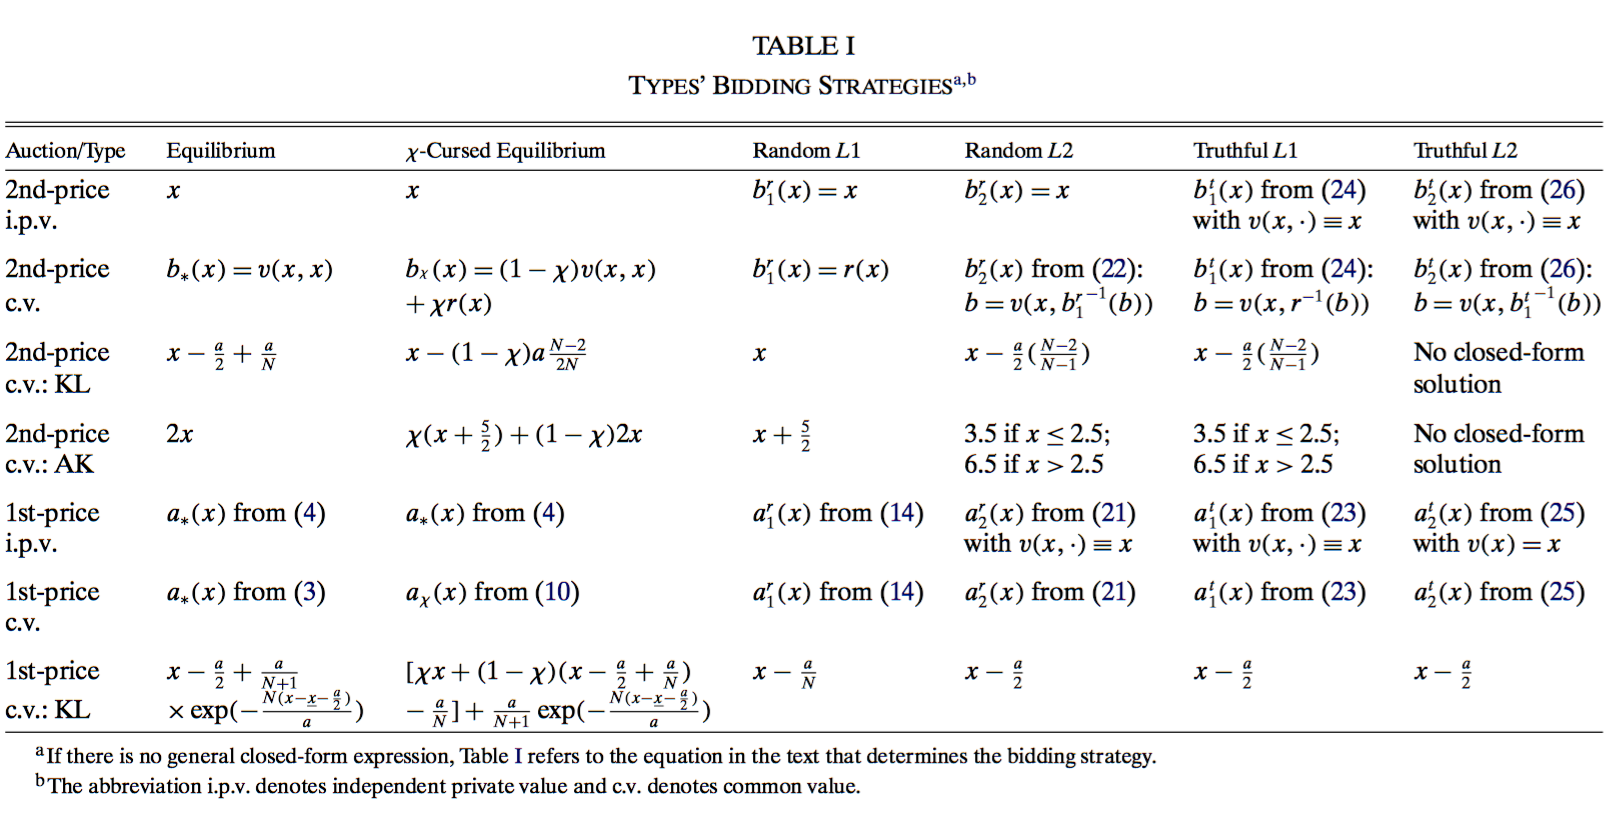
\includegraphics[width = 10cm]{table.png}
		\end{frame}
		
		\begin{frame}\frametitle{Comments on Summary Table}
			\begin{itemize}
			\item In first price independent private value auction (GHP), only bidding trade-off matters.
			\item In second price common value auction (AK), only value adjustment matters.
			\item In first price common value auction (first price version KL), both of them matter in straightforward ways.
			\item The table also includes second price auction version KL example.
			\end{itemize}
		\end{frame}
				
		\begin{frame}[shrink]\frametitle{Level-k Improvements in First Price Auction}
			\begin{itemize}
			\item In i.p.v, when the value is uniformly i.i.d., the equilibrium bidding strategy is a best response to any beliefs derived from others' bidding strategies, therefore L1 and L2 in both of types coincide the equilibrium.
			\item In i.p.v, when the value is distributed nonuniformly, level-k model can explain the overbidding, which is shown in GHP.
			\item In GHP, in high value treatment, Random L1 slightly overbids when he has the highest valuation and Random L2 underbids. Furthermore Truthful L1 overbids while Truthful L2 underbids.
			\item In GHP, in low value treatment, both of Truthful L1 and Truthful L2 underbid, when Random L1 and L2 coincides with equilibrium.
			\item Details are in web appendix.
			\end{itemize}
		\end{frame}
		
		\begin{frame}\frametitle{Level-k Improvements in First Price Auction}
			\begin{itemize}
			\item In c.v, the experiment is KL, both of Random L1 and Random L2 approximately coincide with equilibrium and fully cursed equilibrium biddings when $N = 2$.
			\item When $N > 2$, Random L1 approximately coincides with fully cursed equilibrium bidding, and overbids relative to equilibrium.
			\item When $ N > 2$, value evaluation and bidding trade-off offset each other for both Random L2 and Truthful L1, then they coincide with equilibrium. So does Truthful L2 because it responds to Truthful L1 coinciding with equilibrium.
			\end{itemize}
		\end{frame}
		
		\begin{frame}\frametitle{Level-k Improvements in Second Price Auction}
			\begin{itemize}
			\item In i.p.v, all model have weakly dominant strategies and all players follow them, thus level-k model cannot explain the deviation from equilibrium.
			\item In c.v, both types of level-k model have the potential to explain the deviation.
			\item In KL (with $N > 2$), Random L1 overbids as $N$ and $a$ increase, and random L2 underbids as $N$ decreases and $a$ increases (This is clear from Table 1).
			\end{itemize}
		\end{frame}
		
		\begin{frame}[shrink]\frametitle{Level-k Improvements in Second Price Auction}
			\begin{itemize}
			\item In AK, Random L1 with high signal underbids and one with low signal overbids, since Random L1 bids $r(x)$ in 2nd price auction when $\upsilon(x,x) > r(x)$ for bidders with high signals and $\upsilon(x,x) < r(x)$ for ones with low signals.
			\item In AK, Random L2 with high (low) signal bids the same amount as Random L1 with highest (lowest) possible signal does. 
			\item This is because Random L2 with high signal thinks that other players are Random L1, and so he must win the auction by biding as Random L1 with highest possible signal does. Since $\upsilon(x,x) > r(x)$, the equilibrium expected value of the object is higher than any determined cost. And the same logic can be applied to Random L2 with low signal.
			\end{itemize}
		\end{frame}
		
		\begin{frame}\frametitle{Level-k Improvements in Second Price Auction}
			\begin{itemize}
			\item In KL and AK, Truthful L1 behave as Random L2, since Truthful L0's bidding strategy is identical with the one of Random L1.
			\item In KL, Truthful L2 overbids relative to the cursed equilibrium and increases with N.
			\item In AK, Truthful L2 overbids for some value and underbids for others.
			\item The last two follow from some computations.
			\end{itemize}
		\end{frame}
		
		\begin{frame}\frametitle{Level-k Improvements Summary}
			\begin{itemize}
			\item In 1st price i.p.v (GHP) with nonuniform value, level-k model can improve weakly
			\item In 1st price c.v (KL), Random L1 of level-k model can deviate from equilibrium when $N > 2$.
			\item In 2nd price i.p.v, there is no possibility.
			\item In 2nd price c.v (AK, KL), level-k model has the potential to improve upon cursed equilibrium in both of experiments.
			\end{itemize}
		\end{frame}
		
	\subsection{Econometrical Comparing}
				
		\begin{frame}\frametitle{Preparation for Comparing}
			\begin{itemize}
			\item Because learning can lead even unsophisticated persons to equilibrium, strategic thinking appears most clearly before they see the others' responses. So in this paper they focus on the unexperienced subjects in all the three experiments.
			\item Due to the small sample size, the first 5 responses are regarded as intial responses for each individual.
			\item In first price indipendent private value auction (GHP), the cursed equilibrium coincides with equilibrium, so they use QRE (quantal response equilibrium) instead of cursed equilibrium to explain overbidding.
			\end{itemize}
		\end{frame}
		
		\begin{frame}\frametitle{How to Compare}
			\begin{itemize}
			\item There are three types, i.e. $k$ indexing level-k types ($k = 1,2, \dots, K$), cursed types, and QRE types. And denote each type by $k$.
			\item Denote each game by $g = 1,2,3,4$.
			\item $\lambda_{ik}$ is the logistic error term indexed by subject $i$ and type $k$.
			\item There are three error structures, i.e. the error varying with $i$ and $k$, the error specific to $k$, and the constant error.
			\item $c_{it}^g$ is the observed bidding of subject $i$ in game $g$ at time $t$. And $c_k^g(x)$ is the calculated optimal bidding strategy of the player with type$k$ whose signal is $x$ in game $g$.
			\end{itemize}
		\end{frame}
		
		\begin{frame}\frametitle{How to Compare}
			\begin{itemize}
			\item Let $S_k^g(c | x)$ be the expected payoff of type $k$ player with signal $x$ by bidding $c$ in game $g$, which is defined in advance.
			\item The probability of observing bidding $c$ for type $k$ is computed as follows.
			\end{itemize}
			
			\begin{align}
				Pr(c | k,x,g,\lambda) = \frac{\exp(\lambda S_k^g(c | x))}{\int_{\underline{c}}^{\bar{c}} \exp(\lambda S_k^g(e | x)) \mathrm{d}e}
			\end{align}
		\end{frame}
		
		\begin{frame}\frametitle{How to Compare}
			\begin{itemize}
			\item Let $c_i^g = (c_{i1}^g, c_{i2}^g, c_{i3}^g, c_{i4}^g, c_{i5}^g)$.
			\item Let $\pi_k$ denote the proportion of type $k$ in the population.
			\item With independent errors, by using (26), the type specific likelihood of $c_i^g$ for subject $i$ of type $k$ with signal $x$ and error $\lambda_{ik}$ in game $g$ is (27).
			\item Furthermore the same likelihood unconditional on type is (28).
			\end{itemize}
			
			\begin{align}
				&L_k(c_i^g | k,x,g,\lambda_{ik}) = \Pi_{t = 1}^5 Pr(c_{it}^g | k,x,g,\lambda) \\
				&\sum_{k=1}^K \pi_k L_k(c_i^g | k,x,g,\lambda_{ik}) = \sum_{k=1}^K \pi_k \Pi_{t = 1}^5 Pr(c_{it}^g | k,x,g,\lambda)
			\end{align}
			
		\end{frame}
		
		\begin{frame}\frametitle{How to Compare}
			\begin{itemize}
			\item $N_g$ is the number of subjects in the game $g$.
			\item Let $c^g = (c_1^g, c_2^g, \dots, c_{N_g}^g)$, and the model's likelihood is (29).
			\end{itemize}
			
			\begin{align}
				L(\pi, \Lambda | c^g) = \Pi_{i=1}^{N_g} \sum_{k=1}^K \pi_k L_k(c_i^g | k,x,g,\lambda_{ik})
			\end{align}
		\end{frame}
		
		\begin{frame}\frametitle{Table3a}
			\begin{itemize}
			\item 
			\end{itemize}
		\end{frame}
		
		\begin{frame}\frametitle{Table3c}
			\begin{itemize}
			\item 
			\end{itemize}
		\end{frame}
		
		\begin{frame}\frametitle{Table3d}
			\begin{itemize}
			\item 
			\end{itemize}
		\end{frame}
		
		\begin{frame}\frametitle{Table3b}
			\begin{itemize}
			\item 他と比率が違う理由もかく
			\end{itemize}
		\end{frame}
		
		\begin{frame}\frametitle{Summary: Could Level-k Model really Improve?}
			\begin{itemize}
			\item 
			\end{itemize}
		\end{frame}
	
	
\section{Conclusion}
	\begin{frame}\frametitle{Summary}
		\begin{itemize}
		\item
		\end{itemize}
	\end{frame}
	
	\begin{frame}\frametitle{Implication}
		\begin{itemize}
		\item
		\end{itemize}
	\end{frame}
	

\end{document}
























